\chapter{Knowledge Graph Completion}
\label{cha:knowledge_graph_completion}

As discussed in section \ref{cha:knowledge_graphs} knowledge graphs are not complete. They contain noisy  and incomplete data. It is practically impossible to cover every possible entity and relation existing in the real-world or even in their domain. There might be missing entities and relations or a Knowledge Graph can include two entities/ relations representing the same real-world entity. Knowledge graph completion tries to tackle these and other problems. It can be seen as a way of data cleaning for knowledge graphs. The solutions to the problems are defined into clear tasks, these include: entity resolution and entity and link prediction approaches. \\

\textbf{Entity Resolution} is according to Talburt "the process of determining whether two [entities] are referring to the same object or to different objects". \cite{talburt_entity_2011} \\ 

\textbf{Entity Prediction} is the task of integrating new entities into the knowledge graphs. These entities are are discovered from other external sources and the knowledge graph includes no information about them. The goal is to find all possible relations this new entity has to the entities already existing in the graph. \cite[p.~1]{baumgartner_entity_2021} \\

\textbf{Link Prediction} is quiet similar to entity prediction. Instead of finding links for a new entity the goal here is to find all missing relations between already existing entities. \cite[p.~125]{golbeck_analyzing_2013} Link prediction can be approached in two different ways: entity classification and triple classification. "Entity classification tries to predict the type or the class of an entity [...]" \cite{ilkou_symbolic_2020} For a triple with a missing tail $(h,r,?)$ the goal would be to list all entities which fit into the tail along with their confidence. Triple classification on the other hand is a binary tasks. Here the input is a compete triple $(h,r,t)$ and the goal is to predict whether this triple is true or not. \cite{ilkou_symbolic_2020} \\

In the following we are going to focus on the task of link prediction. There are various models tackling the problem. They can be categorized into one of the following two categories: symbolic and sub-symbolic approaches. While symbolic methods try to learn an explicit symbolic representation of the patterns found in the knowledge graph, sub-symbolic methods try to solve the problem by learning a latent representation, also often referred to as embeddings, for every entity and relation in the knowledge graph. \cite{meilicke_reinforced_2020} 

\section{Symbolic Approaches}
\label{cha:symbolic_methods}

\subsection{AnyBURL}
\label{cha:anyburl}

\section{Sub-Symbolic Approaches}
\label{cha:sub_symbolic_methods}

Sub-symbolic approaches are based on statistics. They try to learn correlations from the existing triples in the knowledge graph. These can then be expressed as a model which in return allows to predict missing facts.  \cite{nickel_review_2016} The most prominent models of this approach are embedding-based models. These models learn a vector for each entity and relation. The resulting embedding then represents our entity or relation. In this representation it is then assumed that similar entities and similar relations will have similar vectors. An example for these embeddings can be seen in figure \ref{fig:embedding_example}. On the left side we see a knowledge graph with three entities and two relations. Every entity and relation are represented on the right side as an embedding. Our two entities \textit{Washington D.C} and \textit{New York City} are both cities and therefore we can assume that their semantical meaning are quiet similar. The embeddings of these two entities are also quiet similar which demonstrates that our previous assumption is correct. \cite{bianchi_knowledge_2021} Our embeddings are also called latent features because they can not be directly observed in the data. Instead our model has to infer these features from the data. \cite{nickel_review_2016} 

\begin{figure}[H]
\centering
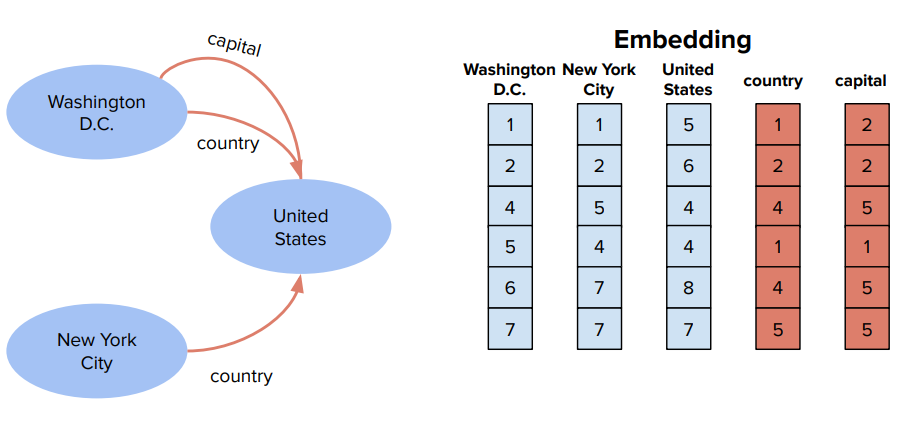
\includegraphics[width=0.9\textwidth]{images/embedding_example.png}
\caption{Example of an Embedding for a Knowledge Graph}
\label{fig:embedding_example}
\end{figure}

An embedding-based model is defined by three characteristics \cite{bianchi_knowledge_2021}:

\begin{enumerate}
\item representations of entities and relationships
\item the scoring function
\item the loss function
\end{enumerate}

As stated earlier our entities and relations are represented through vectors, their embeddings. Some models vary from this a bit and use complex numbers instead of real ones \cite{trouillon_complex_2016}  or use matrices to represent relationships \cite{nickel_three-way_2011}.
\\
The score function $f(h,r,t)$ calculates the distance between the embeddings of two entities relative to their relation. If the triple holds true, its score should be close to $0$. \\
Lastly the loss function defines the objective which is going to be minimized during the training of our model where the embeddings for our entities and relations are learned.

\subsection{ComplEx}
\label{cha:complex}
\subsection{RESCAL}

\section{Comparison of the Approaches}
\label{cha:compare_approaches}

\section{Model Evaluation}
\label{cha:evaluation}